\documentclass[14pt]{extarticle}

\usepackage{fontspec}
\setmainfont{Times New Roman}

% размер полей
\usepackage{geometry}
\geometry{a4paper, top=2cm, bottom=2cm, right=1.5cm, left=3cm}

 %debugging
%\usepackage{showframe}

% полуторный интервал
\usepackage{setspace}
\onehalfspacing

% абзацный отступ
\setlength{\parindent}{1.25cm}

% выравнивание текста по ширине
\sloppy

% списки
\usepackage{calc} % арифметические операции с величинами
\usepackage{enumitem}
\setlist{
    nosep,
    leftmargin=0pt,
    itemindent=\parindent + \labelwidth - \labelsep,
}

% подписи к рисункам и таблицам
\usepackage{caption}
\renewcommand{\figurename}{Рисунок}
\renewcommand{\tablename}{Таблица}
\DeclareCaptionFormat{custom}
{
    \textit{#1#2#3}
}
\DeclareCaptionLabelSeparator{custom}{. }
\captionsetup{
    % хз какой это размер - 12 или нет, но выглядит меньше 14
    font=small,
    format=custom,
    labelsep=custom,
}

% картинки
\usepackage{graphicx}

% колонтитулы
\usepackage{fancyhdr}

% картинки и таблицы находятся именно в том месте текста где помещены (атрибут H)
\usepackage{float}

% таблицы
\usepackage{tabularray}

\graphicspath{ {3.2.3/models/} }
\begin{document}
\pagestyle{fancy}
\fancyhead{}
% disable header
\renewcommand{\headrulewidth}{0pt}
\fancyfoot[L]{Дубровских гр 221-361}
\fancyfoot[C]{ЛР 3.2.3}
\fancyfoot[R]{Продажа автотранспорта}
\singlespacing

\newpage
\begin{center}
    Министерство науки и высшего образования Российской Федерации
    Федеральное государственное автономное образовательное учреждение

    высшего образования

    \guillemotleft МОСКОВСКИЙ ПОЛИТЕХНИЧЕСКИЙ УНИВЕРСИТЕТ\guillemotright

    (МОСКОВСКИЙ ПОЛИТЕХ)
\end{center}
\noindent
\bigbreak
\bigbreak
\bigbreak
\bigbreak
\begin{center}
    ЛАБОРАТОРНАЯ РАБОТА 3.2.3

    По курсу Проектирования пользовательских интерфейсов в веб

    \textbf{Проектирование дизайна веб-страниц низкой точности – каркасов (вайфреймов интерфейса Wireframe)}
    \bigbreak
    \bigbreak
    \bigbreak
    \bigbreak
    ТЕМА

    \guillemotleft\textbf{САЙТ ДЛЯ ПРОДАЖИ И ПОИСКА АВТОМОБИЛЕЙ}\guillemotright
\end{center}
\noindent
\bigbreak
\bigbreak
\bigbreak
\bigbreak
\bigbreak
\bigbreak
\bigbreak
\bigbreak
\bigbreak
\bigbreak
\hfill Выполнил

\hfill Дубровских Никита Евгеньевич

\hfill Группа 221-361
\bigbreak
\bigbreak
\bigbreak
\hfill Проверил

\hfill Натур ВВ
\vfill
\begin{center}
    Москва, 2024
\end{center}
\newpage
\onehalfspacing


\begin{center}
    \textbf{Лабораторная работа 3.2.3}

    \textbf{Проектирование дизайна веб-страниц низкой точности – каркасов (вайфреймов интерфейса Wireframe)}
\end{center}

\textbf{Цель работы:} расположить структурные элементы и блоки страниц на низко детализированном прототипе (вайрфрейме)
\bigskip

\textbf{Задачи:}

\begin{enumerate}
    \item Определить местоположение и размер необходимых элементов внутренней структуры интерфейса  на не менее 10 страницах веб-сайта.
    \item Схематично нарисовать  не менее 5 страниц сайта (каркасов) в черно-белом варианте и указать название всех элементов
    \item Рекомендуется показать переходы (спрогнозировать кликабельность) от элемента к элементу, от страницы к странице (не менее 5 страниц)ю
    \item Дать пояснение месторасположению элементов и блоков страниц с учетом юзабилити, паттерн сканирования, айтрекинга, диаграммы Гутенберга и приемов композиции (Золотое сечение, привило третей, золотая спираль, числа Фибоначчи), как в ЛР «Анализ структуры и основных блоков и элементов страниц веб-сайтов»
\end{enumerate}
\bigskip

\textbf{Основные термины}

\begin{itemize}
    \item Вайрфрейм (Wireframe) - низко детализированный прототип веб-страницы, который показывает расположение элементов интерфейса.
    \item Каркас - аналог термина "вайрфрейм", обозначает структуру страниц сайта.
    \item Прототип - предварительная модель или образец конечного продукта.
    \item Композиция - организация визуальных элементов на странице, включая правила, такие как Золотое сечение, правило третей, золотая спираль и числа Фибоначчи.
    \item Визуальная иерархия - порядок восприятия информации пользователем в зависимости от ее важности.
    \item Линия фолда - граница, разделяющая видимую и невидимую часть веб-страницы при первом взгляде.
\end{itemize}
\bigskip

\textbf{Вайрфреймы}
\bigskip

\noindent
\begin{minipage}{\linewidth}
    
\includegraphics[width=\linewidth]{Header}
    \captionof{figure}{Шапка}
\end{minipage}
\bigskip

\noindent
\begin{minipage}{\linewidth}
    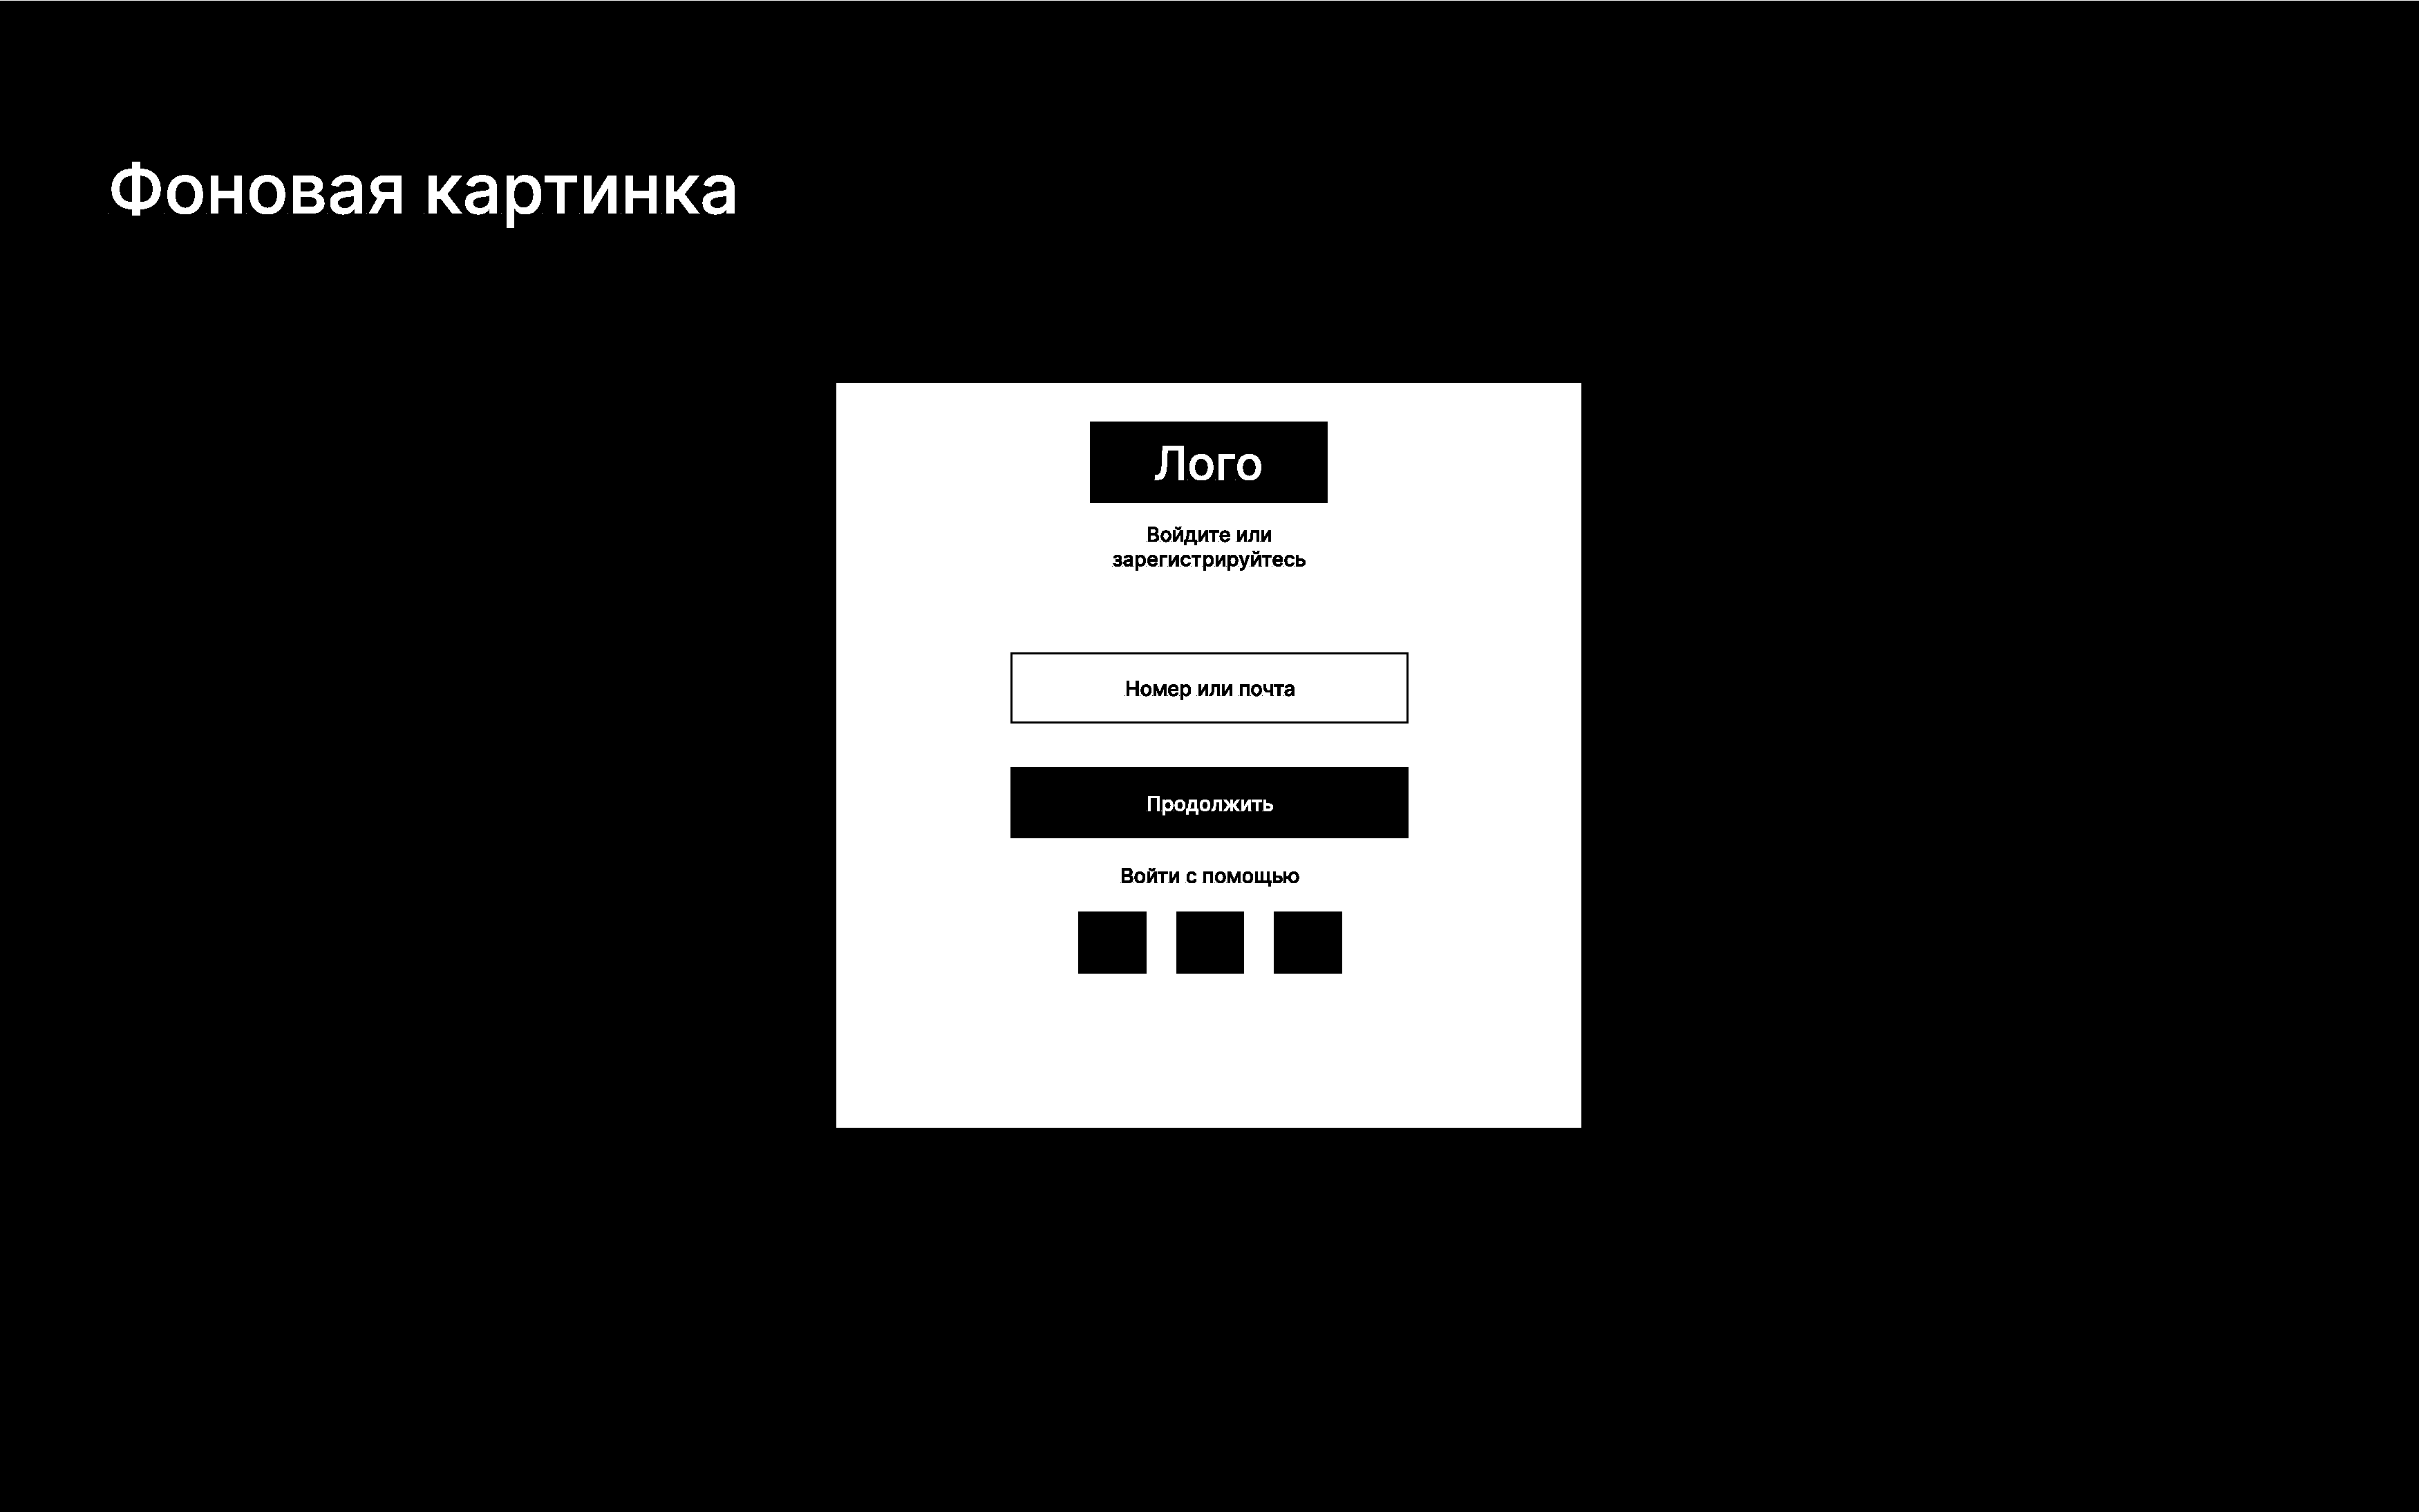
\includegraphics[width=\linewidth]{Auth}
    \captionof{figure}{Авторизация}
\end{minipage}
\bigskip

\noindent
\begin{minipage}{\linewidth}
    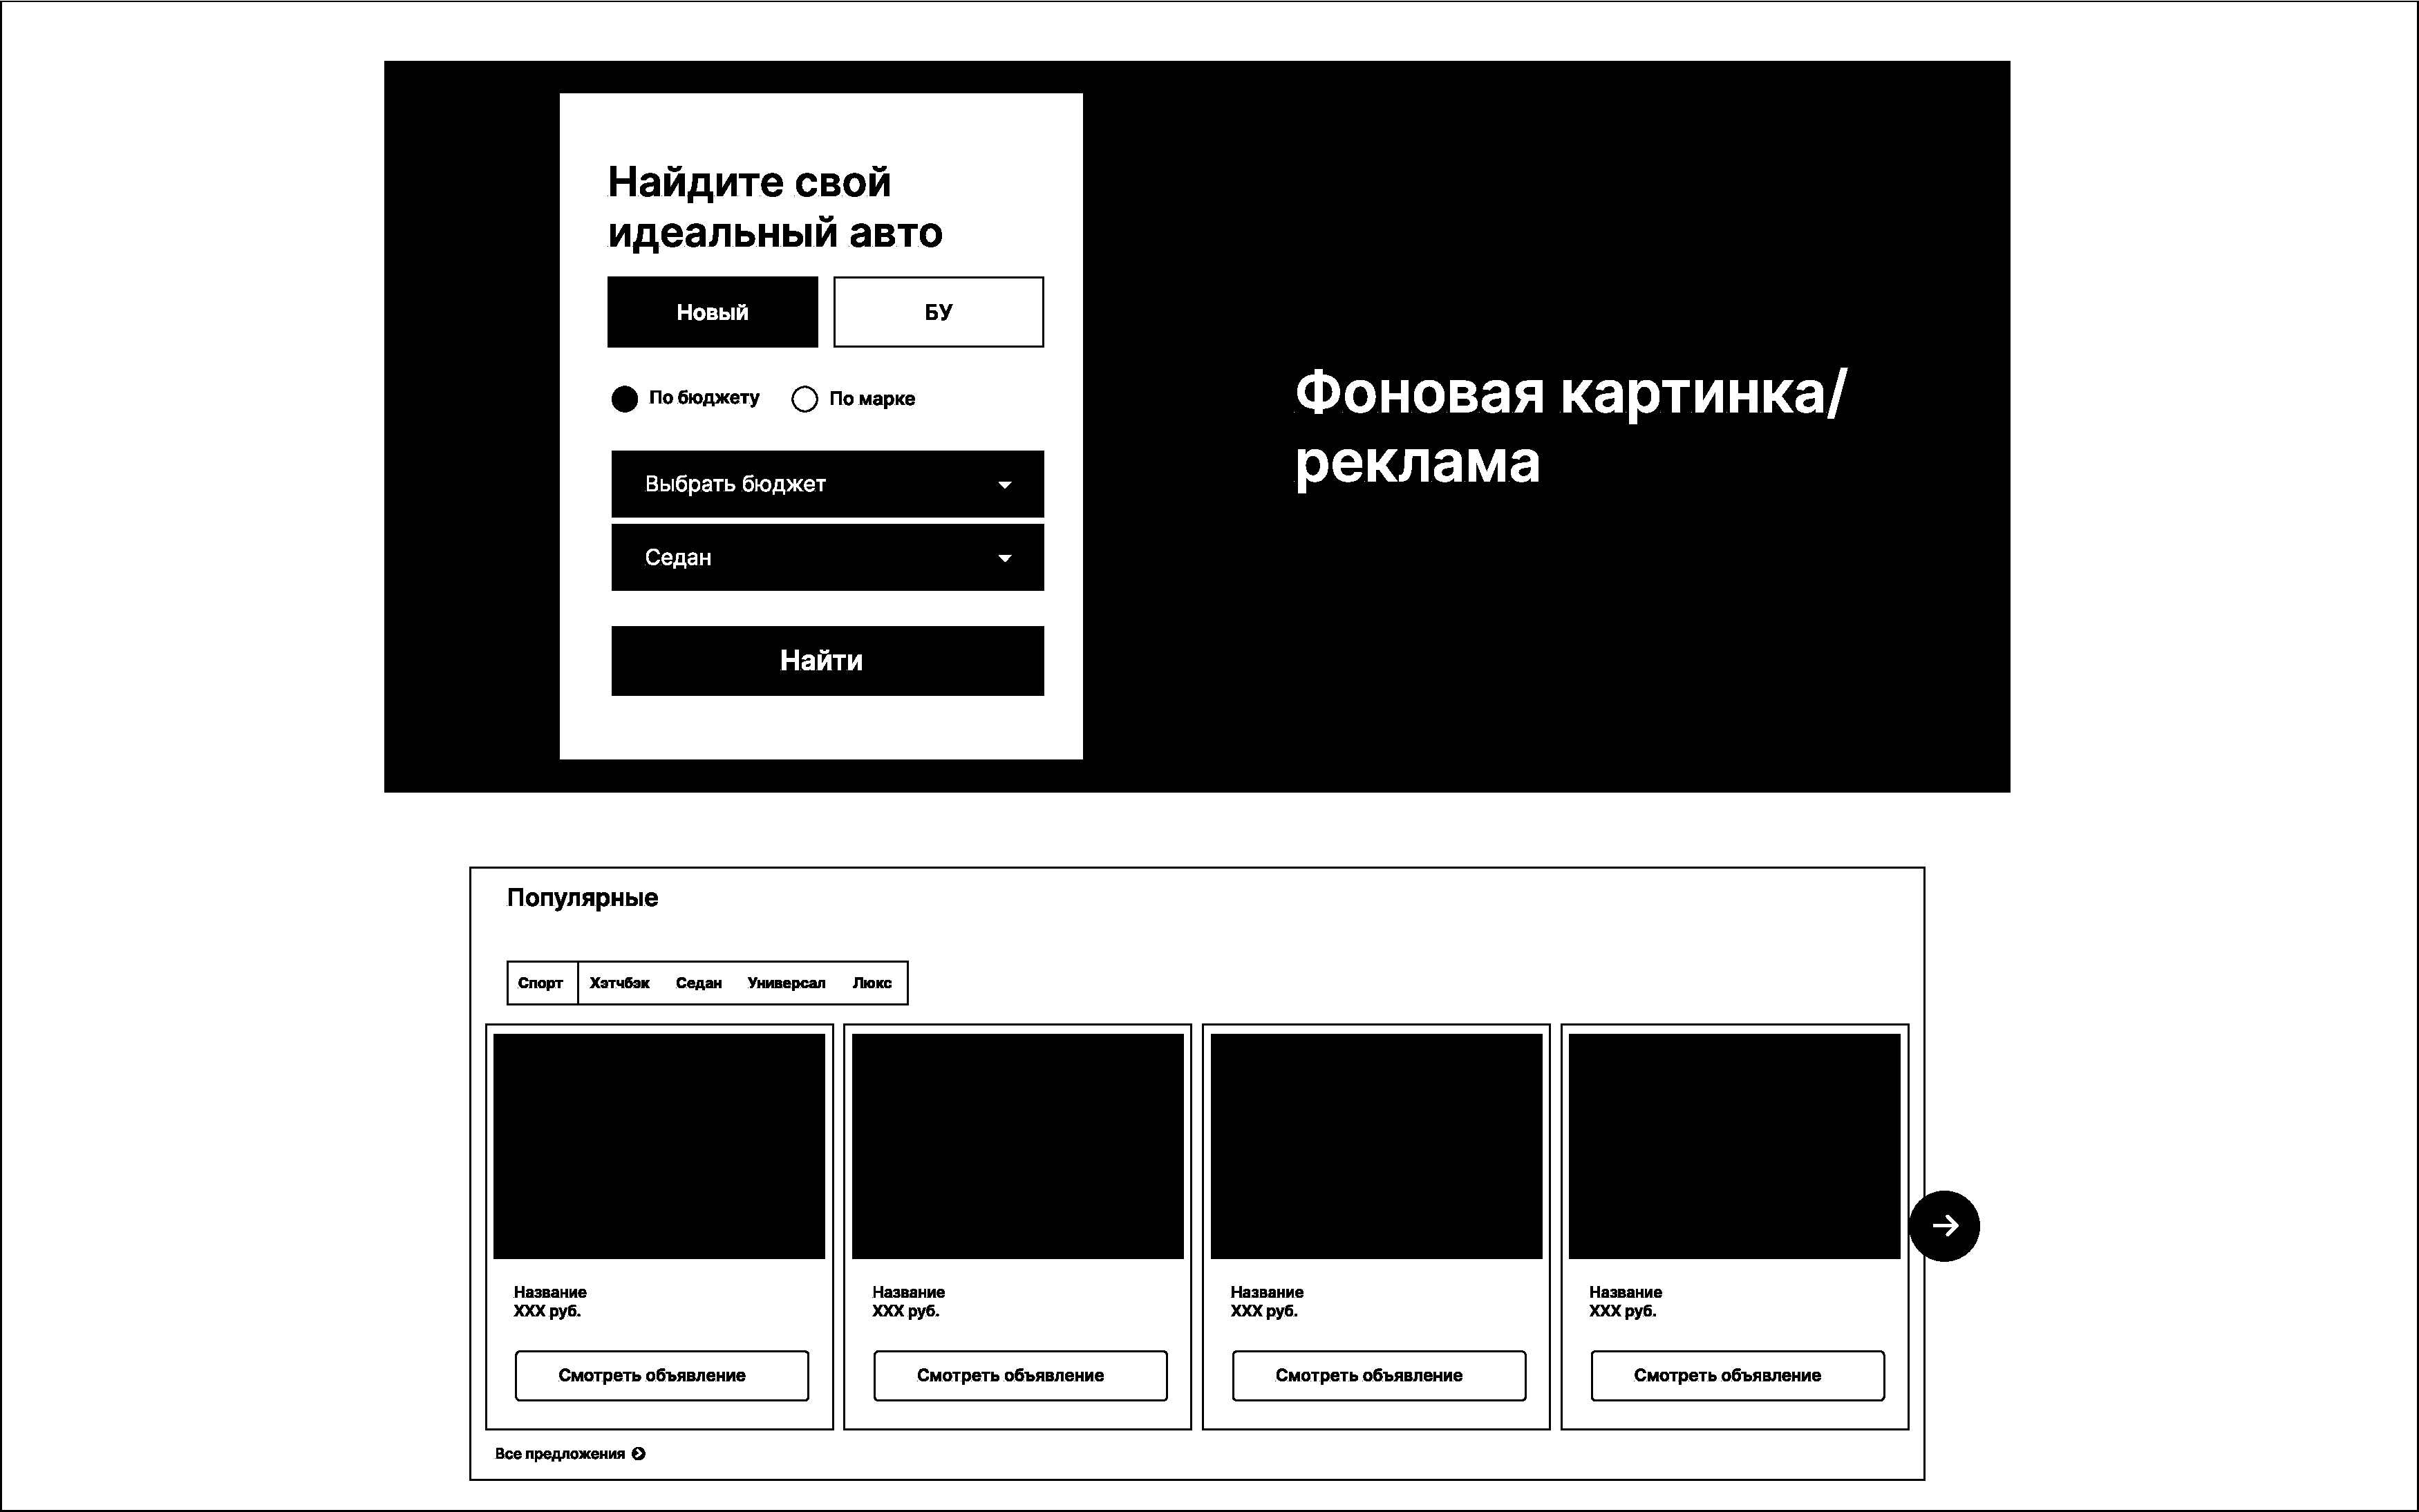
\includegraphics[width=\linewidth]{Main}
    \captionof{figure}{Главная}
\end{minipage}
\bigskip

\noindent
\begin{minipage}{\linewidth}
    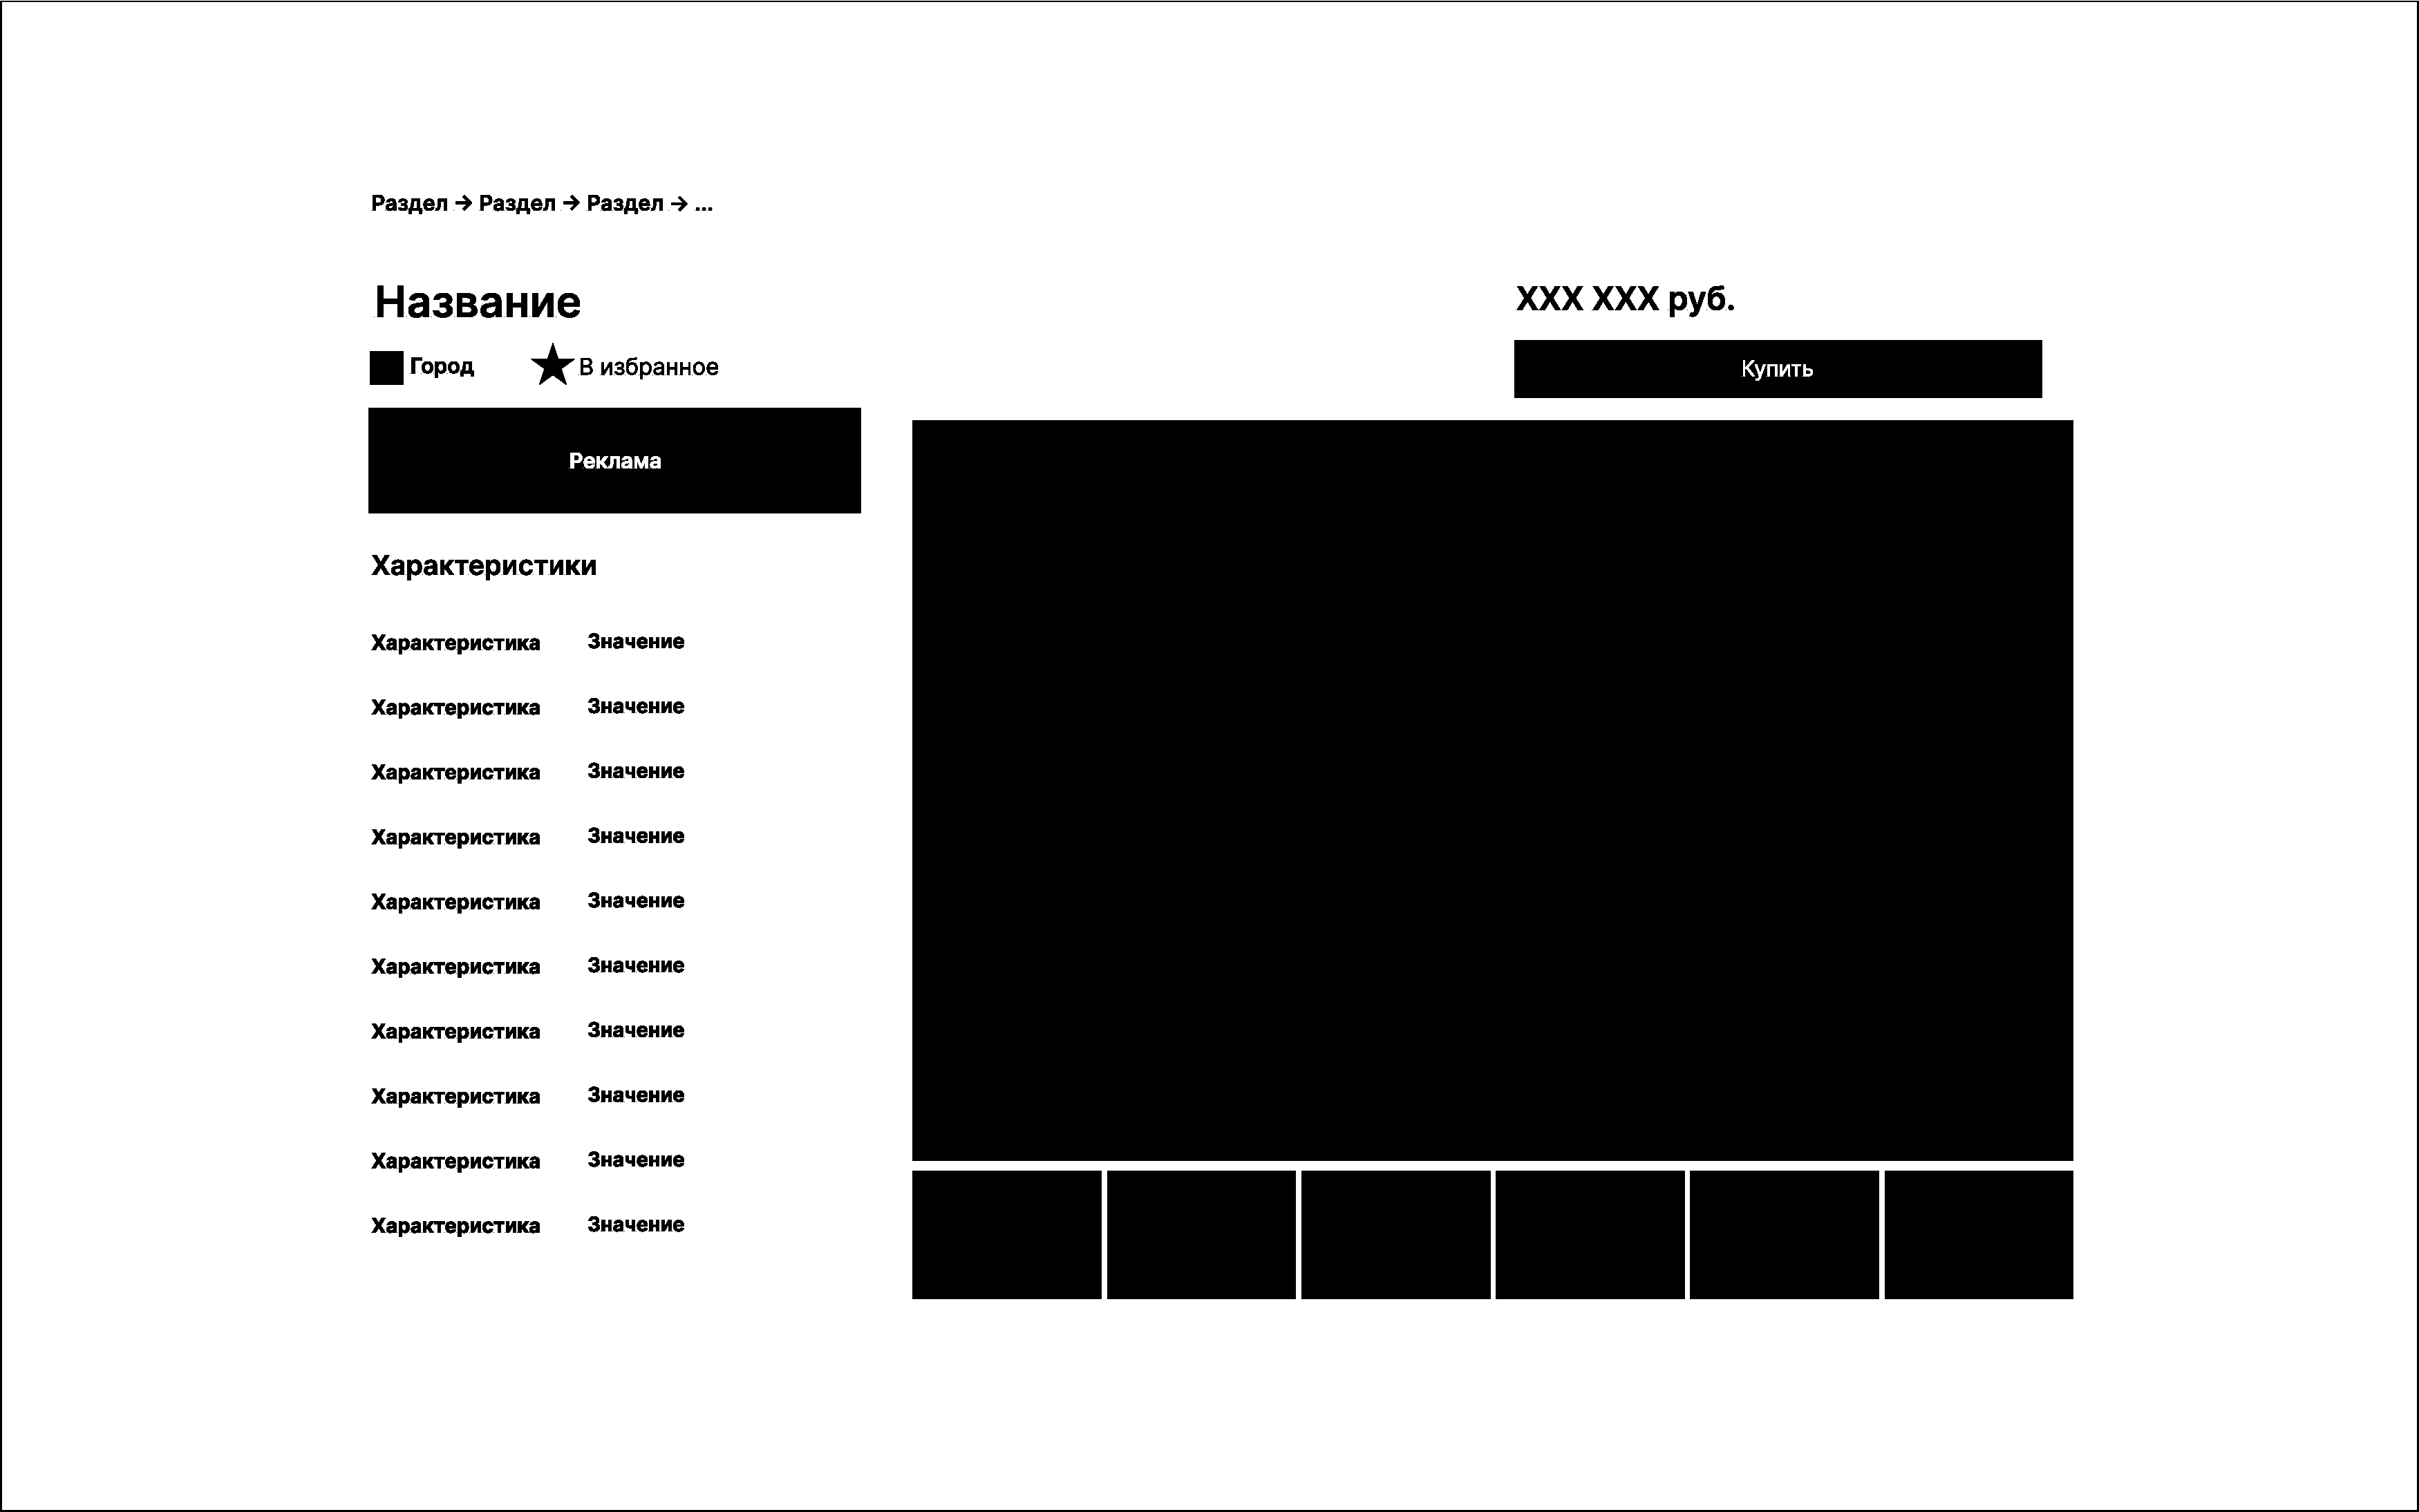
\includegraphics[width=\linewidth]{Selected}
    \captionof{figure}{Выбранный авто}
\end{minipage}
\bigskip

\noindent
\begin{minipage}{\linewidth}
    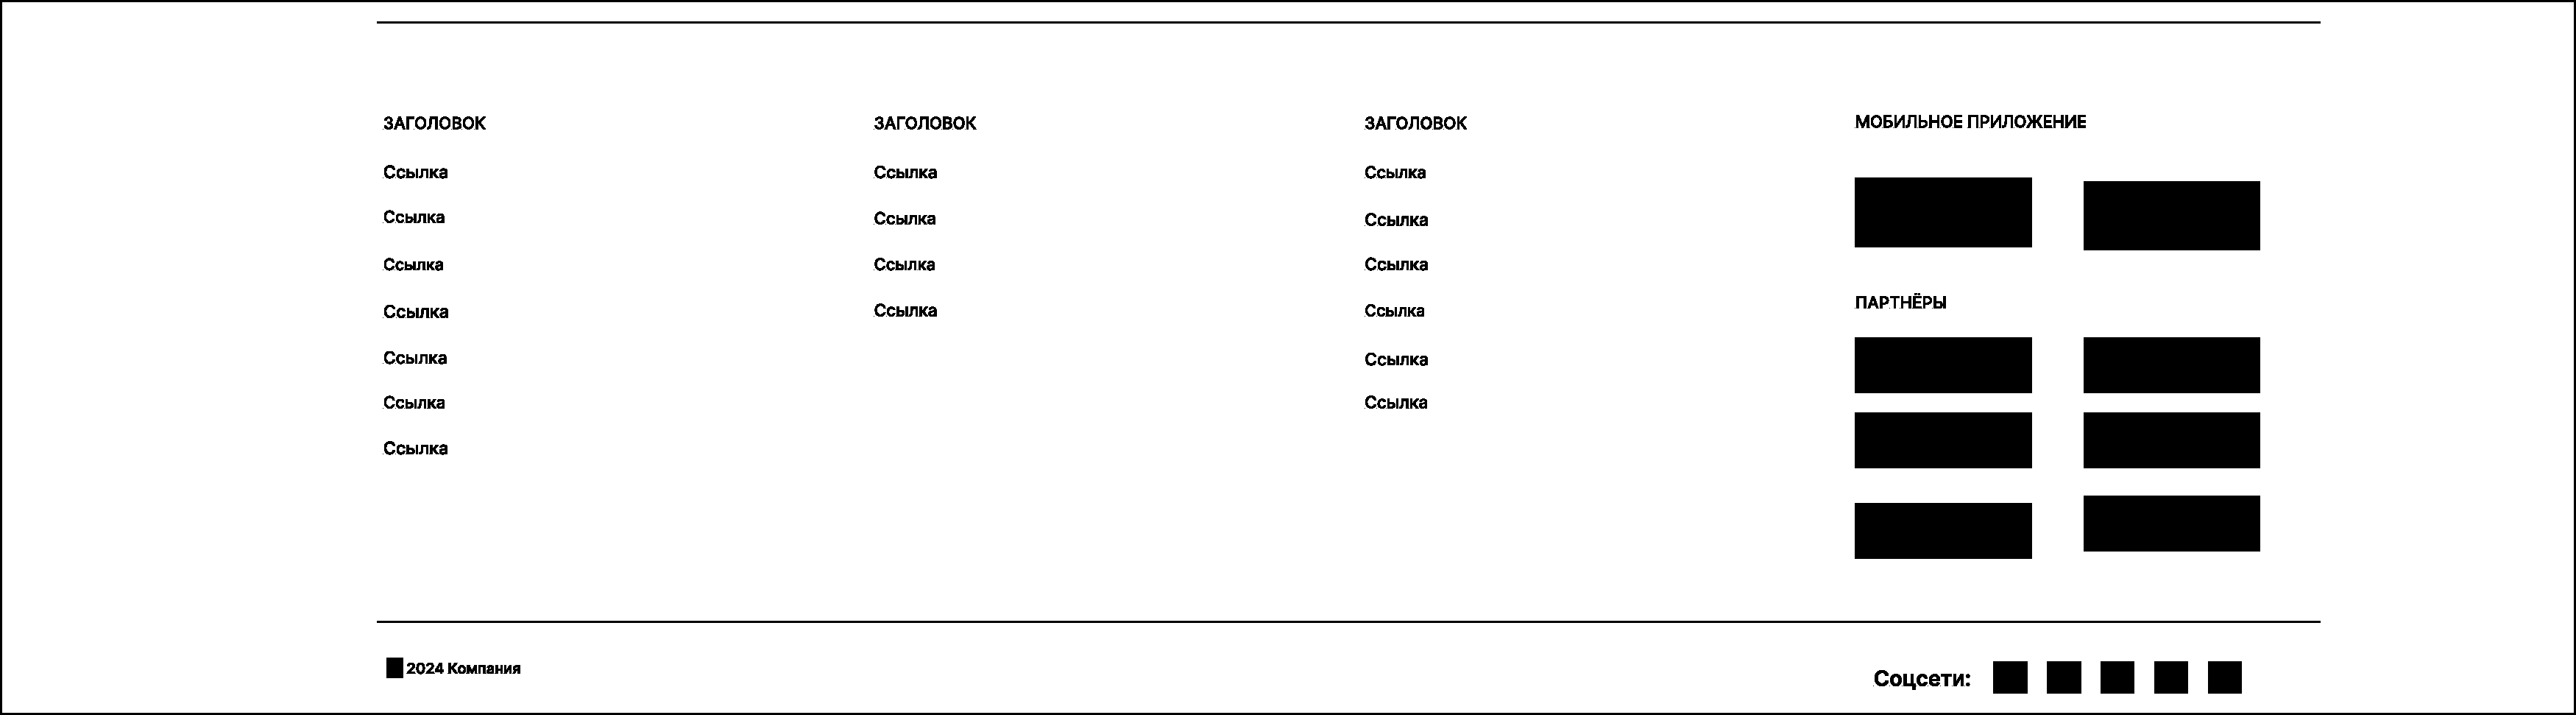
\includegraphics[width=\linewidth]{Footer}
    \captionof{figure}{Подвал}
\end{minipage}
\bigskip

\textbf{Контрольные вопросы и ответы}

\begin{enumerate}
    \item Что такое «вайрфреймы» и зачем они нужны?

    Вайрфреймы (или каркасы) — это низко детализированные прототипы веб-страниц, которые отображают структуру и расположение элементов интерфейса, таких как кнопки, изображения и текст. Они служат для визуализации и планирования дизайна, позволяя команде сосредоточиться на функциональности и пользовательском опыте, прежде чем переходить к более детализированным этапам разработки.
    \item Расскажите про известные вам виды вайрфреймов.

        \begin{itemize}
            \item Низкополигональные вайрфреймы: простые черно-белые схемы, которые показывают базовую структуру страниц.
            \item Среднеполигональные вайрфреймы: более детализированные, могут включать некоторые визуальные элементы и текстовые метки.
            \item Высокополигональные вайрфреймы: почти полноценные прототипы, которые могут включать цвет, шрифты и другие визуальные элементы, но все еще не являются окончательным дизайном.
        \end{itemize}
    \item Как важно располагать элементы страниц?

    Расположение элементов страниц критически важно для удобства использования и восприятия информации пользователями. Правильное размещение помогает пользователям быстро находить нужную информацию, улучшает навигацию и способствует более эффективному взаимодействию с интерфейсом.
    \item Какие правила композиции при расположении элементов рекомендуется учитывать?
        \begin{itemize}
            \item Правило третей: делит страницу на три равные части по горизонтали и вертикали, что помогает создать сбалансированную композицию.
            \item Золотое сечение: пропорция, которая считается эстетически приятной и помогает в размещении элементов.
            \item Гармония и баланс: элементы должны быть сбалансированы по весу и визуальному интересу.
            \item Негативное пространство: использование пустого пространства вокруг элементов для улучшения восприятия и акцентирования внимания.
        \end{itemize}
    \item Принципы визуальной иерархии элементов интерфейса.
        \begin{itemize}
            \item Размер: более крупные элементы привлекают больше внимания.
            \item Цвет: яркие цвета выделяются на фоне более приглушенных.
            \item Близость: элементы, расположенные близко друг к другу, воспринимаются как связанные.
            \item Выравнивание: элементы, выровненные по одной линии, создают порядок и структуру.
            \item Повторение: повторяющиеся стили создают визуальную связь между элементами.
        \end{itemize}
    \item Как в соответствии с F и Z паттернами рекомендуется располагать элементы веб-страниц?
        \begin{itemize}
            \item F-паттерн: пользователи чаще всего сканируют страницы в форме буквы "F", начиная с верхнего левого угла, поэтому важные элементы следует размещать в этих областях.
            \item Z-паттерн: пользователи следуют диагональному пути, который напоминает букву "Z", что позволяет размещать ключевые элементы вдоль этого пути для привлечения внимания.
        \end{itemize}
    \item Какие программы для проектирования вайрфреймов вам известны?
        \begin{itemize}
            \item Figma: популярный инструмент для совместной работы и проектирования интерфейсов.
            \item Sketch: программа для проектирования интерфейсов, особенно популярная среди дизайнеров Mac.
            \item Adobe XD: инструмент для проектирования и прототипирования интерфейсов.
            \item Miro: платформа для совместной работы, которая также поддерживает создание вайрфреймов.
            \item Lucidchart: инструмент для создания диаграмм и вайрфреймов.
            \item draw.io: бесплатный онлайн-сервис для создания диаграмм и вайрфреймов.
        \end{itemize}
    \item Как учитывается линия фолда и область терминала при проектировании интерфейса?

    Линия фолда — это граница, ниже которой пользователи могут не прокручивать страницу. При проектировании интерфейса важно размещать ключевые элементы и информацию выше этой линии, чтобы они были видимы без прокрутки.
\end{enumerate}

\end{document}
